%% LaTeX Beamer presentation template (requires beamer package)
%% see http://latex-beamer.sourceforge.net/
%% idea contributed by H. Turgut Uyar
%% template based on a template by Till Tantau
%% this template is still evolving - it might differ in future releases!

\documentclass[hyperref={pdfpagelabels=false}]{beamer}

\mode<presentation>

% $Id: macros.tex,v 1.4 2013/08/18 16:00:29 ganeshau Exp $
%\usepackage[pdftex]{hyperref}
\frenchspacing
\usepackage{mathptmx}

%\usepackage{cite}
\usepackage[T1]{fontenc}
\usepackage{times}
\usepackage{url}
%\usepackage{cite}
\usepackage{amsmath}
% \usepackage{fancyhdr}
%\usepackage{fancyvrb}
%\usepackage{fancybox}
\usepackage{color}
\usepackage{colortbl}
\usepackage{mathpartir}
\usepackage{amssymb}
\usepackage{xspace}
\usepackage{comment}
\usepackage{graphicx}
\graphicspath{{figures/}}
%\usepackage{epsfig}
%\usepackage{wrapfig}
\usepackage{multirow}
%\usepackage{subfig}

% Added listing for code listings
\usepackage{listings}
\usepackage{relsize}
%\usepackage{stfloats}
\usepackage{fixltx2e}
\usepackage{courier}
% formatting for grammars
% \input{obey}
% \input{grammar}

\usepackage{soul}
\newcommand{\hlc}[2][yellow]{ {\sethlcolor{#1} \hl{#2}} }

%\renewcommand{\nonterm}[1]{\mbox{\textit{#1}}}
\newcommand{\oneormore}[1]{#1\ensuremath{^+}}

% % %\newcommand{\panini}{\textsf{java}$_c$\xspace}
% \newcommand{\mechanism}{active module\xspace}
% \newcommand{\Mechanism}{Active module\xspace}
% \newcommand{\MEchanism}{Active Module\xspace}
% \newcommand{\mechanisms}{active modules\xspace}
% \newcommand{\Mechanisms}{Active modules\xspace}
% \newcommand{\MEchanisms}{Active Modules\xspace}
%\newcommand{\intermechanism}{inter-modular\xspace}
%\newcommand{\intramechanism}{intra-modular\xspace}

\newcommand{\mechanism}{capsule\xspace}
\newcommand{\Mechanism}{Capsule\xspace}
\newcommand{\MEchanism}{Calsupe\xspace}
\newcommand{\mechanisms}{capsules\xspace}
\newcommand{\Mechanisms}{Capsules\xspace}
\newcommand{\MEchanisms}{Capsules\xspace}
\newcommand{\intermechanism}{inter-capsular\xspace}
\newcommand{\intramechanism}{intra-capsular\xspace}

\newcommand{\MRB}{Message Ring Buffer\xspace}
\newcommand{\mrb}{message ring buffer\xspace}
\newcommand{\TaskFramework}{task framework\xspace}

% Type checking macros
% change symbol type of : from mathrel 
%\DeclareMathSymbol{:}{\mathbin}{operators}{"3A} 
\newcommand{\OK}{\mbox{OK}}
\newcommand{\OKin}{\mbox{OK in }}
\newcommand{\inC}{\mbox{in }c}
\newcommand{\isType}{\mbox{\textit{isType}}}
\newcommand{\validFields}{\mbox{\textit{validF}}}
\newcommand{\isClass}{\mbox{\textit{isClass}}}
\newcommand{\isHandler}{\mbox{\textit{isHandler}}}
\newcommand{\Types}{\mbox{\textit{Types}}}
\newcommand{\Names}{\mbox{\textit{Names}}}
\newcommand{\TypeEnv}{\mbox{\textit{TypeEnv}}}
\newcommand*{\findMeth}{\auxFunc{findMeth}}
\newcommand*{\fieldsOf}{\auxFunc{fields}}
\newcommand*{\fieldName}{\auxFunc{fieldName}}
\newcommand*{\checkMethods}{\auxFunc{methE}}
\newcommand*{\methodEffect}{\auxFunc{me}}
\newcommand*{\typeOfField}{\auxFunc{typeOfF}}
\newcommand*{\typeOf}{\auxFunc{typeOf}}
\newcommand*{\dom}{\auxFunc{dom}}
\newcommand*{\rng}{\auxFunc{rng}}
\newcommand*{\isAnn}{\auxFunc{annotated}}
\newcommand*{\updateEffect}{\auxFunc{update}}
\newcommand*{\reversePointer}{\auxFunc{reverse}}
\newcommand*{\reversePoint}{\auxFunc{reverseP}}
\newcommand*{\fixPoint}{\auxFunc{fixPoint}}
\newcommand*{\updateOther}{\auxFunc{updateOther}}
\newcommand*{\updateMethodEffect}{\auxFunc{updateEff}}
\newcommand*{\updateSingleMethodEffect}{\auxFunc{updateMeth}}
\newcommand*{\updateSingleEffect}{\auxFunc{concretize}}
\newcommand*{\updateForkEffect}{\auxFunc{updateFork}}
\newcommand*{\updateQueue}{\auxFunc{updateQ}}
\newcommand*{\getActive}{\auxFunc{active}\xspace}
\newcommand*{\field}{\auxFunc{field}}
\newcommand{\fdecl}{\mbox{\textit{fdecl}}}
\newcommand*{\fieldOf}{\auxFunc{fieldOf}}
\newcommand*{\getOpen}{\auxFunc{getOpen}}
\newcommand{\NPE}{\mbox{\textit{NPE}}}

% Reserved words (in math mode)
\newcommand{\Extends}{\mbox{\texttt{\textbf{extends}}}}
\newcommand{\Implements}{\mbox{\texttt{\textbf{implements}}}}
\newcommand{\This}{\mbox{\texttt{\textbf{this}}}}
\newcommand{\Self}{\mbox{\texttt{\textbf{self}}}}
\newcommand{\EV}{\mbox{\texttt{\textbf{event}}~}}
\newcommand{\Cast}{\mbox{\texttt{\textbf{cast}}}}
\newcommand{\New}{\mbox{\texttt{\textbf{new}}~}}
\newcommand{\Null}{\mbox{\texttt{\textbf{null}}}}
\newcommand{\Chain}{\mbox{\texttt{\textbf{chain}}~}}
\newcommand{\Under}{\mbox{\texttt{\textbf{under}}~}}
\newcommand{\If}{\mbox{\texttt{\textbf{if}}}}
\newcommand{\Then}{\mbox{\texttt{\textbf{then}}}}
\newcommand{\Else}{\mbox{\texttt{\textbf{else}}}}
\newcommand{\While}{\mbox{\texttt{\textbf{while}}}}

% Aux functions
\newcommand{\auxFunc}[1]{\ensuremath{\mathop{\mathit{#1}}}}
\newcommand*{\override}{\auxFunc{override}}

% types
\newcommand{\POWERSET}[1]{\mbox{\textit{PowerSet}}(#1)}
\newcommand{\delete}{\mbox{\textit{delete}}}
\newcommand{\mklist}{\mbox{\textit{mksupers}}}
\newcommand{\uminus}{\mbox{$\cup\!\!\!\!-$}}
\newcommand{\iminus}{\mbox{$\cap\!\!\!\!-$}}
\newcommand{\commutesWith}{\sharp}
\newcommand{\notCommutesWith}{\not\sharp}
\newcommand{\rname}[1]{$\TirName{(#1)}$} % for inline inferrule names
\newcommand{\STO}{\ensuremath{<:}}  % ``subtype of''
\newcommand{\notSTO}{\ensuremath{\not<:}}  % ``subtype of''
\newcommand{\consistent}{\ensuremath{\approx}}

% auxiliary funtions for finding the dynamic effects for program executions.
\newcommand*{\dynamicInfinite}{\auxFunc{dynValue}}
\newcommand*{\dynamicEffects}{\auxFunc{dynE}}
\newcommand*{\dynamicEffectsOnce}{\auxFunc{dyn}}
\newcommand*{\dynamicEffectSet}{\auxFunc{dynESet}}
\newcommand*{\predecessorSiblings}{\auxFunc{preS}}
\newcommand*{\predSibles}{\auxFunc{pSib}}
%\newcommand*{\offspring}{\auxFunc{descendentsOf}}
%\newcommand*{\offspring}{\auxFunc{descendents}}
\newcommand*{\offspring}{\auxFunc{desc}}
\newcommand*{\offspringOrItself}{\auxFunc{descendOrSelf}} 
\newcommand*{\inQueueX}{\auxFunc{inQ}} 
\newcommand*{\inQueueY}{\auxFunc{inq}}
\newcommand*{\replaceQueue}{\auxFunc{replace}}
\newcommand*{\substituteSequence}{\auxFunc{subSeq}}
\newcommand*{\combineSequence}{\auxFunc{comSeq}}
\newcommand*{\mergeSequence}{\auxFunc{merSeq}}
\newcommand*{\isin}{\auxFunc{belongs}}
\newcommand*{\configuration}{c}

% Macros for operational semantics
\newcommand{\mc}[1]{\mbox{\rm \ensuremath{\text{\code{#1}}}}} % Arg set in code font in math
\newcommand{\loc}{\ensuremath{\mathord{\mathit{loc}}}}
\newcommand{\handler}[3]{\ensuremath{\langle#1,#2,#3\rangle}}
\newcommand{\ec}{\ensuremath{\mathbb{E}}}
%\newcommand{\ec}{\ensuremath{\mathop{\mathbb{E}}}}
%\newcommand{\ecpending}{\ensuremath{\mathop{\mathbb{E'}}}}
\newcommand{\ecpending}{\ensuremath{\mathop{\overline{\mathbb{E}}}}}
\newcommand{\hole}{\ensuremath{\mathord{\mathit{-}}}}
\newcommand{\reducesto}{\hookrightarrow}
\newcommand{\reducestostar}{\overset{*}{\reducesto}}
\newcommand{\dontcare}{\ensuremath{\mathord{\text{\textvisiblespace\hspace{0.10ex}}}}}
\newcommand{\Expression}{\ensuremath{{\cal E}}}
\newcommand{\Stack}{\mbox{\textit{Stack}}}
\newcommand{\Store}{\mbox{\textit{Store}}}
\newcommand{\ActiveList}{\mbox{\textit{ActiveList}}}
\newcommand{\Frame}{\mbox{\textit{Frame}}}
\newcommand{\FieldEnv}{\mbox{\textit{FieldEnv}}}
\newcommand{\ObjectRecord}{\mbox{\textit{ObjectRecord}}}
\newcommand{\lexframe}{\mbox{\textbf{\texttt{frame}}}}
\newcommand{\handlerframe}{\mbox{\textbf{\texttt{hframe}}}}
\newcommand{\Excep}{\mbox{\textit{Excep}}}

\newcommand*{\seq}[1]{\ensuremath{\left\langle {#1} \right\rangle}} % Arg is sequence contents
\newcommand{\config}{\seq}
\newcommand{\udot}{\mathbin{\sqcup \kern-0.53em \cdot \,}}

\newcommand{\eseq}{\hat{e}}

% Effect attributes
\newcommand{\ReadE}{\mbox{\texttt{\textbf{read}}~}}
%\newcommand{\WriteE}{\mbox{\texttt{\textbf{write}}~}}
\newcommand{\WriteE}{\mbox{\texttt{\textbf{write}}~}}
\newcommand{\CheckE}{\mbox{\texttt{\textbf{open}}}}
%\newcommand{\ForkE}{\mbox{\texttt{\textbf{fork}}}}
\newcommand{\ForkE}{\mbox{\texttt{\textbf{fork}}}}
\newcommand{\EnqueueE}{\mbox{\texttt{\textbf{bottom}}}}
%\newcommand{\BottomE}{\mbox{\texttt{\textbf{\bot}}}}
\newcommand{\RegisterE}{\mbox{\texttt{\textbf{exp}}}}
%\newcommand{\AnnounceE}{\mbox{\texttt{\textbf{frk}}~}}
\newcommand{\CreateE}{\mbox{\texttt{\textbf{create}}~}}
% Effect Auxiliary Functions
\newcommand*{\EffectsOf}{\auxFunc{effects}}
\newcommand{\ReadF}{\mbox{\texttt{\textbf{rd}}}}
\newcommand{\WriteF}{\mbox{\texttt{\textbf{wt}}}}
\newcommand{\ForkF}{\mbox{\texttt{\textbf{fk}}}}
\newcommand{\EnqueueF}{\mbox{\texttt{\textbf{eq}}}}
\newcommand{\BottomF}{\mbox{\texttt{\textbf{bt}}}}
\newcommand{\ConcretizedF}{\mbox{\texttt{\textbf{ct}}}}
\newcommand{\OtherF}{\mbox{\texttt{\textbf{el}}}}


\newcommand{\Class}{\mbox{\texttt{\textbf{class}}~}}
\newcommand{\tasks}{\mbox{\texttt{\textbf{tasks}}~}}
\newcommand{\fork}{\mbox{\texttt{\textbf{fork}}~}}
\newcommand{\foreach}{\mbox{\texttt{\textbf{forall}}~}}
\newcommand{\Decl}{\mbox{\texttt{\textbf{decl}}~}}
\newcommand{\RDecl}{\mbox{\texttt{\textbf{rdecl}}~}}
\newcommand{\Exp}{\mbox{\texttt{\textbf{exp}}~}}
\newcommand{\Prog}{\mbox{\texttt{\textbf{prog}}~}}
\newcommand{\Meth}{\mbox{\texttt{\textbf{meth}}~}}
\newcommand{\Type}{\mbox{\texttt{\textbf{type}}}}
\newcommand{\var}{\mbox{\textit{var}}}
\newcommand{\Nil}{\ensuremath{\bullet}}
%\newcommand{\st}{\ensuremath{\textrm{s.t.}}}
\newcommand{\true}{\ensuremath{\mathit{true}}}
\newcommand{\false}{\ensuremath{\mathit{false}}}
\newcommand{\Land}{\ensuremath{\bigwedge}}

% New Panini features
\newcommand{\Announce}{\mbox{\texttt{\textbf{announce}}~}}
\newcommand{\Yield}{\mbox{\texttt{\textbf{yield}}~}}
%\newcommand{\Future}{\mbox{\texttt{\textbf{Future}}~}}

\newcommand{\When}{\mbox{\texttt{\textbf{when}}}}
\newcommand{\Do}{\mbox{\texttt{\textbf{do}}}}
\newcommand{\Return}{\mbox{\texttt{\textbf{return}}}}
\newcommand{\Invoke}{\mbox{\texttt{\textbf{invoke}}}}
\newcommand{\Thunk}{\mbox{\texttt{\textbf{thunk}}~}}
\newcommand{\Register}{\mbox{\texttt{\textbf{register}}}}
\newcommand{\EventClosure}{\mbox{\texttt{\textbf{eClosure}}}}
\newcommand{\Boolean}{\mbox{\texttt{\textbf{boolean}}}}
\newcommand{\Int}{\mbox{\texttt{\textbf{int}}}}
\newcommand{\Void}{\mbox{\texttt{\textbf{void}}}}
\newcommand{\Nat}{\mbox{\texttt{\textbf{Nat}}}}

% auxiliary funtions for updating the event hierarchies
%\newcommand*{\updateGamma}{\auxFunc{updateHierarchy}}
\newcommand*{\updateGamma}{\auxFunc{updateHier}}
\newcommand*{\inGamma}{\auxFunc{registered}}
\newcommand*{\inDelta}{\auxFunc{inHierarchy}}
\newcommand*{\inZeta}{\auxFunc{inList}}
%\newcommand*{\updateEffect}{\auxFunc{updateEffect}}
\newcommand*{\collectBindings}{\auxFunc{colEvts}}
\newcommand*{\collectEvents}{\auxFunc{colEvt}}
\newcommand*{\putEvent}{\auxFunc{putEvent}}
\newcommand*{\putHierarchies}{\auxFunc{putHierarchies}}
\newcommand*{\putLevel}{\auxFunc{putLevel}}
\newcommand*{\effectsHierachy}{\auxFunc{effHier}}
\newcommand*{\effectsList}{\auxFunc{effList}}
\newcommand*{\effectsUnion}{\auxFunc{effUn}}
\newcommand*{\mergeRho}{\auxFunc{mergeRho}}
\newcommand*{\mergeEpsilon}{\auxFunc{mergeEff}}
\newcommand*{\effectEnlarge}{\auxFunc{effectEnlarge}}
\newcommand*{\insertLast}{\auxFunc{insert}}
\newcommand*{\compareLast}{\auxFunc{comp}}
\newcommand*{\build}{\auxFunc{build}}
\newcommand*{\isConcurrent}{\auxFunc{parallel}}
\newcommand*{\conflict}{\auxFunc{disjointMeth}}
\newcommand*{\disjoint}{\auxFunc{disj}}
\newcommand*{\interfere}{\auxFunc{nonConfl}}
\newcommand*{\deepCopy}{\auxFunc{copy}}
\newcommand*{\findMax}{\auxFunc{fresh}}
\newcommand*{\forkTask}{\auxFunc{buildconfs}}
\newcommand*{\intersect}{\auxFunc{intersect}}
\newcommand*{\inQueue}{\auxFunc{inQueue}}
\newcommand*{\copyEffect}{\auxFunc{cp}}
\newcommand*{\getTask}{\auxFunc{getTask}}
\newcommand*{\getFirstTask}{\auxFunc{getfirst}}

\definecolor{Brown}{cmyk}{0,0.81,1,0.60}
\definecolor{OliveGreen}{cmyk}{0.64,0,0.95,0.40}
\definecolor{CadetBlue}{cmyk}{0.62,0.57,0.23,0}
\definecolor{lightlightgray}{gray}{0.9}

\definecolor{lightest-gray}{rgb}{0.95,0.95,0.5}
\definecolor{lighter-gray}{rgb}{0.7,0.98,0.7}
\definecolor{light-gray}{rgb}{0.5,0.98,0.98}
%\definecolor{light-gray}{rgb}{0.0,0.75,0.80}
\definecolor{dark-gray}{rgb}{0.95,0.7,0.95}
\definecolor{darker-gray}{rgb}{1,0.65,0.65}

% settings for listings
\definecolor{white}{gray}{1.0}
\definecolor{lightergray}{gray}{0.99}
\definecolor{lightgray}{gray}{0.97}
\definecolor{darkgray}{gray}{0.5}
\definecolor{OliveGreen}{cmyk}{0.64,0,0.95,0.40}

\lstset{
	language={[Visual]Basic}, emph={},
	mathescape=false, escapechar=@,
	backgroundcolor=\color{lightgray},
	commentstyle=\color{darkgray},
	keywordstyle=\color{OliveGreen}\bfseries,
	basicstyle=\scriptsize\sffamily,
	numberstyle=\scriptsize\sffamily,
	emphstyle=\bfseries,
	numbers=left, stepnumber=1,
	numberblanklines=false,
	numberstyle=\tiny,
	numbersep=-3pt,
	frame=none, framexleftmargin=0pt, framexrightmargin=0pt, 
	%xleftmargin=15pt, xrightmargin=4pt,
	columns=flexible, breaklines=true,
	showspaces=false, showstringspaces=false, showtabs=false, tabsize=2,
	morekeywords={abstract,case,catch,class,def,do,else,extends,%
          false,final,finally,for,forSome,if,implicit,import,lazy,%
          match,new,null,object,override,package,private,protected,%
          return,sealed,super,this,throw,trait,true,try,type,%
          val,var,while,with,yield,
          map,filter,flatmap,sample,groupByKey,reduceByKey,
          union,join,cogroup,crossProduct,mapValues,sort,partitionBy,
          count,collect,reduce,lookup,save},
	otherkeywords={=>,<-,<\%,<:,>:,\#,@}
}

% could use \relsize{-2} instead of \scriptsize below
\newcommand{\FIGCODEFONT}{\relsize{-1}\ttfamily}
\newcommand{\FIGCODELIBFONT}{\relsize{-6}\ttfamily}

% cross referencing
\newcommand{\figref}[1]{Figure~\ref{#1}}
\newcommand{\tabref}[1]{Table~\ref{#1}}
\newcommand{\fignref}[1]{Figure~\ref{#1}}
\newcommand{\appref}[1]{Appendix~\ref{#1}}
\newcommand{\secref}[1]{\S\ref{#1}}
\newcommand{\secnref}[1]{\S\ref{#1}}
\newcommand{\defref}[1]{Definition~\ref{#1}}
\newcommand{\lemref}[1]{Lemma~\ref{#1}}
\newcommand{\theref}[1]{Theorem~\ref{#1}}
\newcommand{\lineref}[1]{line~\ref{#1}}
\newcommand{\linesref}[2]{lines~\ref{#1}-\ref{#2}}
\newcommand{\linerefNum}[1]{\ref{#1}}
\newcommand{\footnoteref}[1]{$^{\ref{#1}}$}

%  % {theorems}
%  \newtheorem{theorem}{Theorem}[section]
%  \newtheorem{axiom}[theorem]{Axiom}
%  \newtheorem{corollary}[theorem]{Corollary}
%  \newtheorem{definition}[theorem]{Definition}
%  \newtheorem{example}[theorem]{Example}
%  \newtheorem{fact}[theorem]{Fact}
%  \newtheorem{lemma}[theorem]{Lemma}
%  \newtheorem{proposition}[theorem]{Proposition}
%  \newtheorem{remark}[theorem]{Remark}
%  \newtheorem{conjecture}[theorem]{Conjecture}

%Some helpful notation
\newcommand{\PROOF}{{\em Proof:\/}~~}

\newcommand{\etal}{~\textit{et al.}}

%\newcommand{\PROOFSKETCH}{{\em Proof Sketch:\/}~~}
\newcommand{\PROOFSKETCH}{{\em Proof:\/}~~}
%\newcommand{\QED}{\rule{0.4em}{0.65em}}

\newcommand\para[1]{\vspace{0.1em}{\bf #1.}\ }
%\newcommand\para[1]{\paragraph{#1}}

% formatting of initial section quotations
\newcommand{\QUOTATION}[1]{\begin{scriptsize}\begin{flushright}\emph{#1}\end{flushright}\end{scriptsize}}

% \newtheorem{theorem}{{\bf Theorem}}[section]
% \newenvironment{definition}[1][Definition]{\begin{trivlist}
% \item[\hskip \labelsep {\bfseries #1}]}{\end{trivlist}}
% 
% \newenvironment{lemma}[1][Lemma]{\begin{trivlist}
% \item[\hskip \labelsep {\bfseries #1}]}{\end{trivlist}}
% 
% \newenvironment{example}[1][Example]{\begin{trivlist}
% \item[\hskip \labelsep {\bfseries #1}]}{\end{trivlist}}
% 
% \newenvironment{remark}[1][Remark]{\begin{trivlist}
% \item[\hskip \labelsep {\bfseries #1}]}{\end{trivlist}}

% \newcommand{\qed}{\nobreak \ifvmode \relax \else
%       \ifdim\lastskip<1.5em \hskip-\lastskip
%       \hskip1.5em plus0em minus0.5em \fi \nobreak
%       \vrule height0.75em width0.5em depth0.25em\fi}

% Allow figures to take up the entire page
\renewcommand\floatpagefraction{.99}
\renewcommand\topfraction{.99}
\renewcommand\bottomfraction{.90}
\renewcommand\textfraction{.01}

% \renewcommand{\topfraction}{0.90}
% \renewcommand{\textfraction}{0.05}
% \renewcommand{\floatpagefraction}{0.85}

\usepackage{graphicx}
\usetheme{isu}
\usepackage{times}
\usepackage{amsmath,amsthm, amssymb, latexsym}
\boldmath
\usepackage[english]{babel}
\usepackage[latin1]{inputenc}
\usepackage{listings}

\DeclareGraphicsExtensions{.pdf,.jpg,.png}
\graphicspath{{figures/}}

\title[641 Project]{Concurrent Graph Mutation: A static approach to handle graph topology mutation conflicts}
\author[Team Bliss]{Bliss
\linebreak Team Member(s):
\linebreak Aashish Dhakal
\linebreak Eric Lin
\linebreak Samantha S. Khairunnesa}
\institute[ISU]{Department of Computer Science \linebreak Iowa State
University}

\date[COMS 641]{COMS 641: Data Intensive Languages and Systems - Design and Semantics}
%\date{Month X, 20XX}

% If you have a file called "university-logo-filename.xxx", where xxx
% is a graphic format that can be processed by latex or pdflatex,
% resp., then you can add a logo as follows:

%\pgfdeclareimage[height=0.25cm]{logo}{figures/logo}
%\logo{\pgfuseimage{logo}}


\begin{document}
  \begin{frame}[plain]
    \titlepage
  \end{frame}
  \section{Problem}
% TODO What is the problem and why do we care

\subsection{Background}

\begin{frame}
\begin{itemize}
  \item Many problems in scientific computing, data mining and other domains are leading to graph algorithm specific soltuions
  \item Growth of these problems (e.g. Web Graph and various social networks) asks for parallel computing resources.
  \item Some of the algorithms requires a combination of vertex-centric (parallel) and global (sequential) computations. 
  	\begin{itemize}
	 \item An example could be k-means-like graph clustering algorithm.
	 \end{itemize}
  \item This type of algorithm requires a means of graph mutation operations.
    	\begin{itemize}
		\item Eg: Giraph, Mizan, GPS, Graph Lab (supports partial mutation)
	\end{itemize}
\end{itemize}	
\end{frame}

\subsection{Context}	

\begin{frame}
  	\begin{itemize}
		\item However, topology mutation operations performed concurrently at different vertices can conflict with each other
  \linebreak
  \item Pregel tries to resolve mutation conflicts by using:
  	  	\begin{itemize}
			\item Partial ordering
			\item User defined handlers
			\linebreak
		\end{itemize}
  \item Users need to have prior knowledge regarding ordering of mutation and conflicts that may occur
  \end{itemize}
\end{frame}

\begin{frame}
\begin{itemize}
  \item Correctness partial ordering.
  \linebreak
  \item Design a detection technique to identify the all the conflicts that may occur while minimizing the false positives.
  \linebreak
  \item How to provide a better abstraction to enable means of an unambiguous mutation of graph topology?
\end{itemize}
\end{frame}


  \section{Examples}
\subsection{Problem example}
\begin{frame}[fragile]
\begin{lstlisting}[
    language=Java]
  public interface Computation<I, V, E, M>{
    void compute(Vertex<I,V,E> vertex, Iterable<M> messages);
    //Must be defined by user to do computation on a single Vertex.
	
    void 	addEdgeRequest(I sourceVertexId, Edge<I,E> edge);
    void 	addVertexRequest(I id, V value);
    void 	removeEdgesRequest(I sourceVertexId, I targetVertexId);
    void 	removeVertexRequest(I vertexId);
    long 	getSuperstep();
    long 	getTotalNumEdges();
    long 	getTotalNumVertices();
    void 	postSuperstep();
    void 	preSuperstep();
    void 	sendMessage(I id, M message);
  }
\end{lstlisting}
Essential operations of a \textit{Computation} in Giraph
\end{frame}

\begin{frame}[fragile]
\begin{lstlisting}[
    language=Java]
  Public class SimpleMutateGraphComputation extends BasicComputation<
    LongWritable, DoubleWritable, FloatWritable, DoubleWritable> {

    public void compute(Vertex<LongWritable, DoubleWritable, FloatWritable>
      vertex, Iterable<DoubleWritable> messages){ 
      if (getSuperstep() == 0) {
      	addVertexRequest(getVertexCount(), new
      	DoubleWritable(vertex.getValue()));
      } else if (getSuperstep() == 1) {
        vertex.voteToHalt();
    } 
  }
\end{lstlisting}
Example of a program that mutates a graph
\end{frame}

  \section{Solution}

\subsection{Analysis on the Conflicts}

\begin{frame}
	1. Analysis to detect conflicts
	\begin{itemize}
		\item Possible combinations introducing conflicts
		\linebreak
			\begin{figure}
			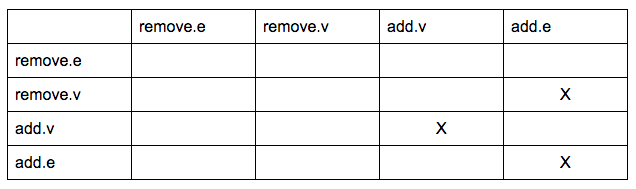
\includegraphics[width=0.8\linewidth]{figures/table.jpg}
			\caption{Combination that creates conflicts}
			\end{figure}
	\end{itemize}
\end{frame}

\begin{frame}	
		 \begin{itemize}
		      \item Refinement of the analysis
		      \linebreak
		   	  \begin{itemize}
				\item Look at the compute() of active vertices in a Superstep 
				\item Collect topology mutation operations
				\item Prune the list if the operation in consideration does not fall into any categories that create conflicts
				\item Take control and data flow into consideration
				\item Formally model the graph mutation and use a proof assistant to prove the correctness of the process
		     	  \end{itemize}
		  \end{itemize}
\end{frame}

\begin{frame}[fragile]
\begin{lstlisting}[
    language=Java]
  Public class SimpleMutateGraphComputation extends BasicComputation<
    LongWritable, DoubleWritable, FloatWritable, DoubleWritable> {

    public void compute(Vertex<LongWritable, DoubleWritable, FloatWritable>
      vertex, Iterable<DoubleWritable> messages){ 
      if (getSuperstep() == 0) {
      	addVertexRequest(getVertexCount(), new
      	DoubleWritable(vertex.getValue()));
      } else if (getSuperstep() == 1) {
        vertex.voteToHalt();
    } 
  }
\end{lstlisting}
Example of a program that mutates a graph
\end{frame}

\begin{frame}	

2. Handle conflicts by abstraction
		      \linebreak
		   	  \begin{itemize}
				\item There are some conflicts that can not be solved by partial ordering 
				\item User defined handlers are suggested to resolve such issues.
				\item Current mechanism is writing user defined handlers to randomly select one of the operation that introduces conflicts.
				\item A better abstraction can add priority to handlers to help decide the operation to be performed if there is a conflict.
		     	  \end{itemize}

\end{frame}



  \section{Evaluation Method}
\begin{frame}
Our two goals:
  	\begin{itemize}
		 \item The soundness of our analysis to detect conflicting mutation
		 \item The completeness of resolving conflicting mutation with the
		 existence of required handlers
    \end{itemize}
    Evaluating our solutions by applying it on graph processing platform
    benchmarks:
    \begin{itemize}
		 \item Graphalytics
		 \item Graph500
    \end{itemize}
\end{frame}

\begin{frame}
 We also plan to model graph transformations in proof assistants to
 provide a formal proof of the soundness of out solutions \linebreak
\begin{itemize}
  \item Formalizing graphs and graph transformation
  \item Formalizing our analysis 
  \item Martin Strecker., "Modeling and Verifying Graph Transformations in
  Proof Assistants", ENTCS, Vol. 203 Issue 1, 2008
\end{itemize}

\end{frame}

 
  \section{Other Problems}
\subsection{Other Problems 1}
\begin{frame}
One main contribution of FlumeJava is the optimization of execution plan by
reordering the data operations. For example, ParallelDo operations are fused,
related GroupByKey operations are combined by analyzing the data flow.
\begin{itemize}
  \item Correctness of the optimization is not described
  \item Same for many optimization techniques that is used in many frameworks
  seen in the course
  \item Also similar to the problem we picked, but more specific to single
  techniques in specific framework.
\end{itemize}
\end{frame}

\subsection{Other Problems 2}
\begin{frame}
A problem mentioned in the FlumeJava paper is that the abstraction of
operations make it easier for programmers to write MapReduce programs, but the
abstraction also causes programers to write program that is logical to them but
is inefficient. The inefficiency is caused by the lack of understanding of the
underlying execution.
\begin{itemize}
  \item This can be optimized by having a better analysis to remove redundant
  operations
  \item Very specific analysis for a specific framework and difficult to apply
  to other works.
\end{itemize}
\end{frame}

\subsection{Picked Problem}
\begin{frame}
\begin{itemize}
  \item The picked problem explores concurrent graph mutation in a concurrent context,
which can be applied to following works on concurrent graph processing
  \item Graph processing have always been an important class of problems that
  can be used applied to many real world problems
  \item Work on concurrent graph processing can be more broadly applied, and may
  be more interesting to broader audience.
\end{itemize}
\end{frame}
  \section{Related Works}
\subsection{Closely related works}

\begin{frame}
\begin{itemize}
  \item Pregel provides the topology mutation feature to facilitate graph algorithms such as clustering algorithm, minimum spanning tree.
  \item Although it provides partial ordering to achieve determinism, yet forces the programmer to understand the reordering to close the gap between the logic of the programmer and what actually happens to effectively resolve conflicts that are not solved by partial ordering.
  \item Pregel-like frameworks such as Giraph, GPS, Mizan, and GraphLab supports graph mutations, yet do not address the conflicts arising due to concurrent topology mutation.
  \end{itemize}
   \let\thefootnote\relax\footnotetext{\tiny[Minyang et. el., "An Experimental Comparison of Pregel-like Graph Processing Systems", VLDB, Vol. 7 Issue 12, 2014]}
\end{frame}

\begin{frame}
	\begin{itemize}
	\item Martin et. al. formalized the graph transformation based on set-theoretic model.
	\item In the paper, it is mentioned that the graph transformation should specify the condition under which it will be applicable and the action needs to be taken at a position in a source graph to obtain target graph.
	\item They do not map graphs into graphs, as in traditional graph rewriting, rather verify that the applicability condition of a transformation rule is true
  	\end{itemize}
  \let\thefootnote\relax\footnotetext{\tiny[Martin Strecker., "Modeling and Verifying Graph Transformations in Proof Assistants", ENTCS, Vol. 203 Issue 1, 2008]}
\end{frame} 

\begin{frame}
	\begin{itemize}
	 \item They have also claimed application of well-formed graph transformations to well-formed graphs yields again well-formed graphs.
	 \item This kind of formalization has not been yet utilized to address the correctness of partial ordering.
  	\end{itemize}
  \let\thefootnote\relax\footnotetext{\tiny[Martin Strecker., "Modeling and Verifying Graph Transformations in Proof Assistants", ENTCS, Vol. 203 Issue 1, 2008]}
\end{frame} 


\subsection{More related works}
\begin{frame}
\begin{itemize}

\item Serafettin Tasci and Murat Demirbas, "Giraphx: Parallel Yet Serializable Large-Scale Graph Processing", EuroPar, 2013. 
\item Joseph E. Gonzalez, Yucheng Low, Haijie Gu, Danny Bickson, Carlos Guestrin, "PowerGraph: Distributed Graph-Parallel Computation on Natural Graphs", OSDI, 2012.     
\item Zuhair Khayyat, Karim Awara, Amani Alonazi, Hani Jamjoom, Dan Williams, and Panos Kalnis, "Mizan: A System for Dynamic Load Balancing in Large-scale Graph Processing" ACM EuroSys, 2013. 
Zuhair Mizan 
    \end{itemize}
\end{frame}
 
\begin{frame}
\begin{itemize}
\item Semih Salihoglu and Jennifer Widom, "GPS: A Graph Processing System", Proc. International Conference on Scientific and Statistical Database Management (SSDBM), 2013.
 \item Yucheng Low, Joseph Gonzalez, Aapo Kyrola, Danny Bickson, Carlos Guestrin, and Joseph M. Hellerstein, "GraphLab: A New Parallel Framework for Machine Learning, In Uncertainty in Artificial Intelligence, 2010.
\item U Kang, Charalampos E. Tsourakakis, and Christos Faloutsos, PEGASUS: A Peta-Scale Graph Mining System Implementation and Observations, IEEE International Conference on Data Mining (ICDM), 2009.
    \end{itemize}
\end{frame}


\begin{frame}
\begin{itemize}
\item Zechao Shang, and Jeffrey Xu Yu, "Catch the Wind: Graph workload balancing on cloud Data Engineering", IEEE 29th International Conference in Data Engineering, 2013.
    \end{itemize}
\end{frame}
\end{document}
